\documentclass[tikz,border=6pt]{standalone}
\usepackage{amsmath,amssymb}
\usetikzlibrary{calc,arrows.meta,positioning}

\begin{document}
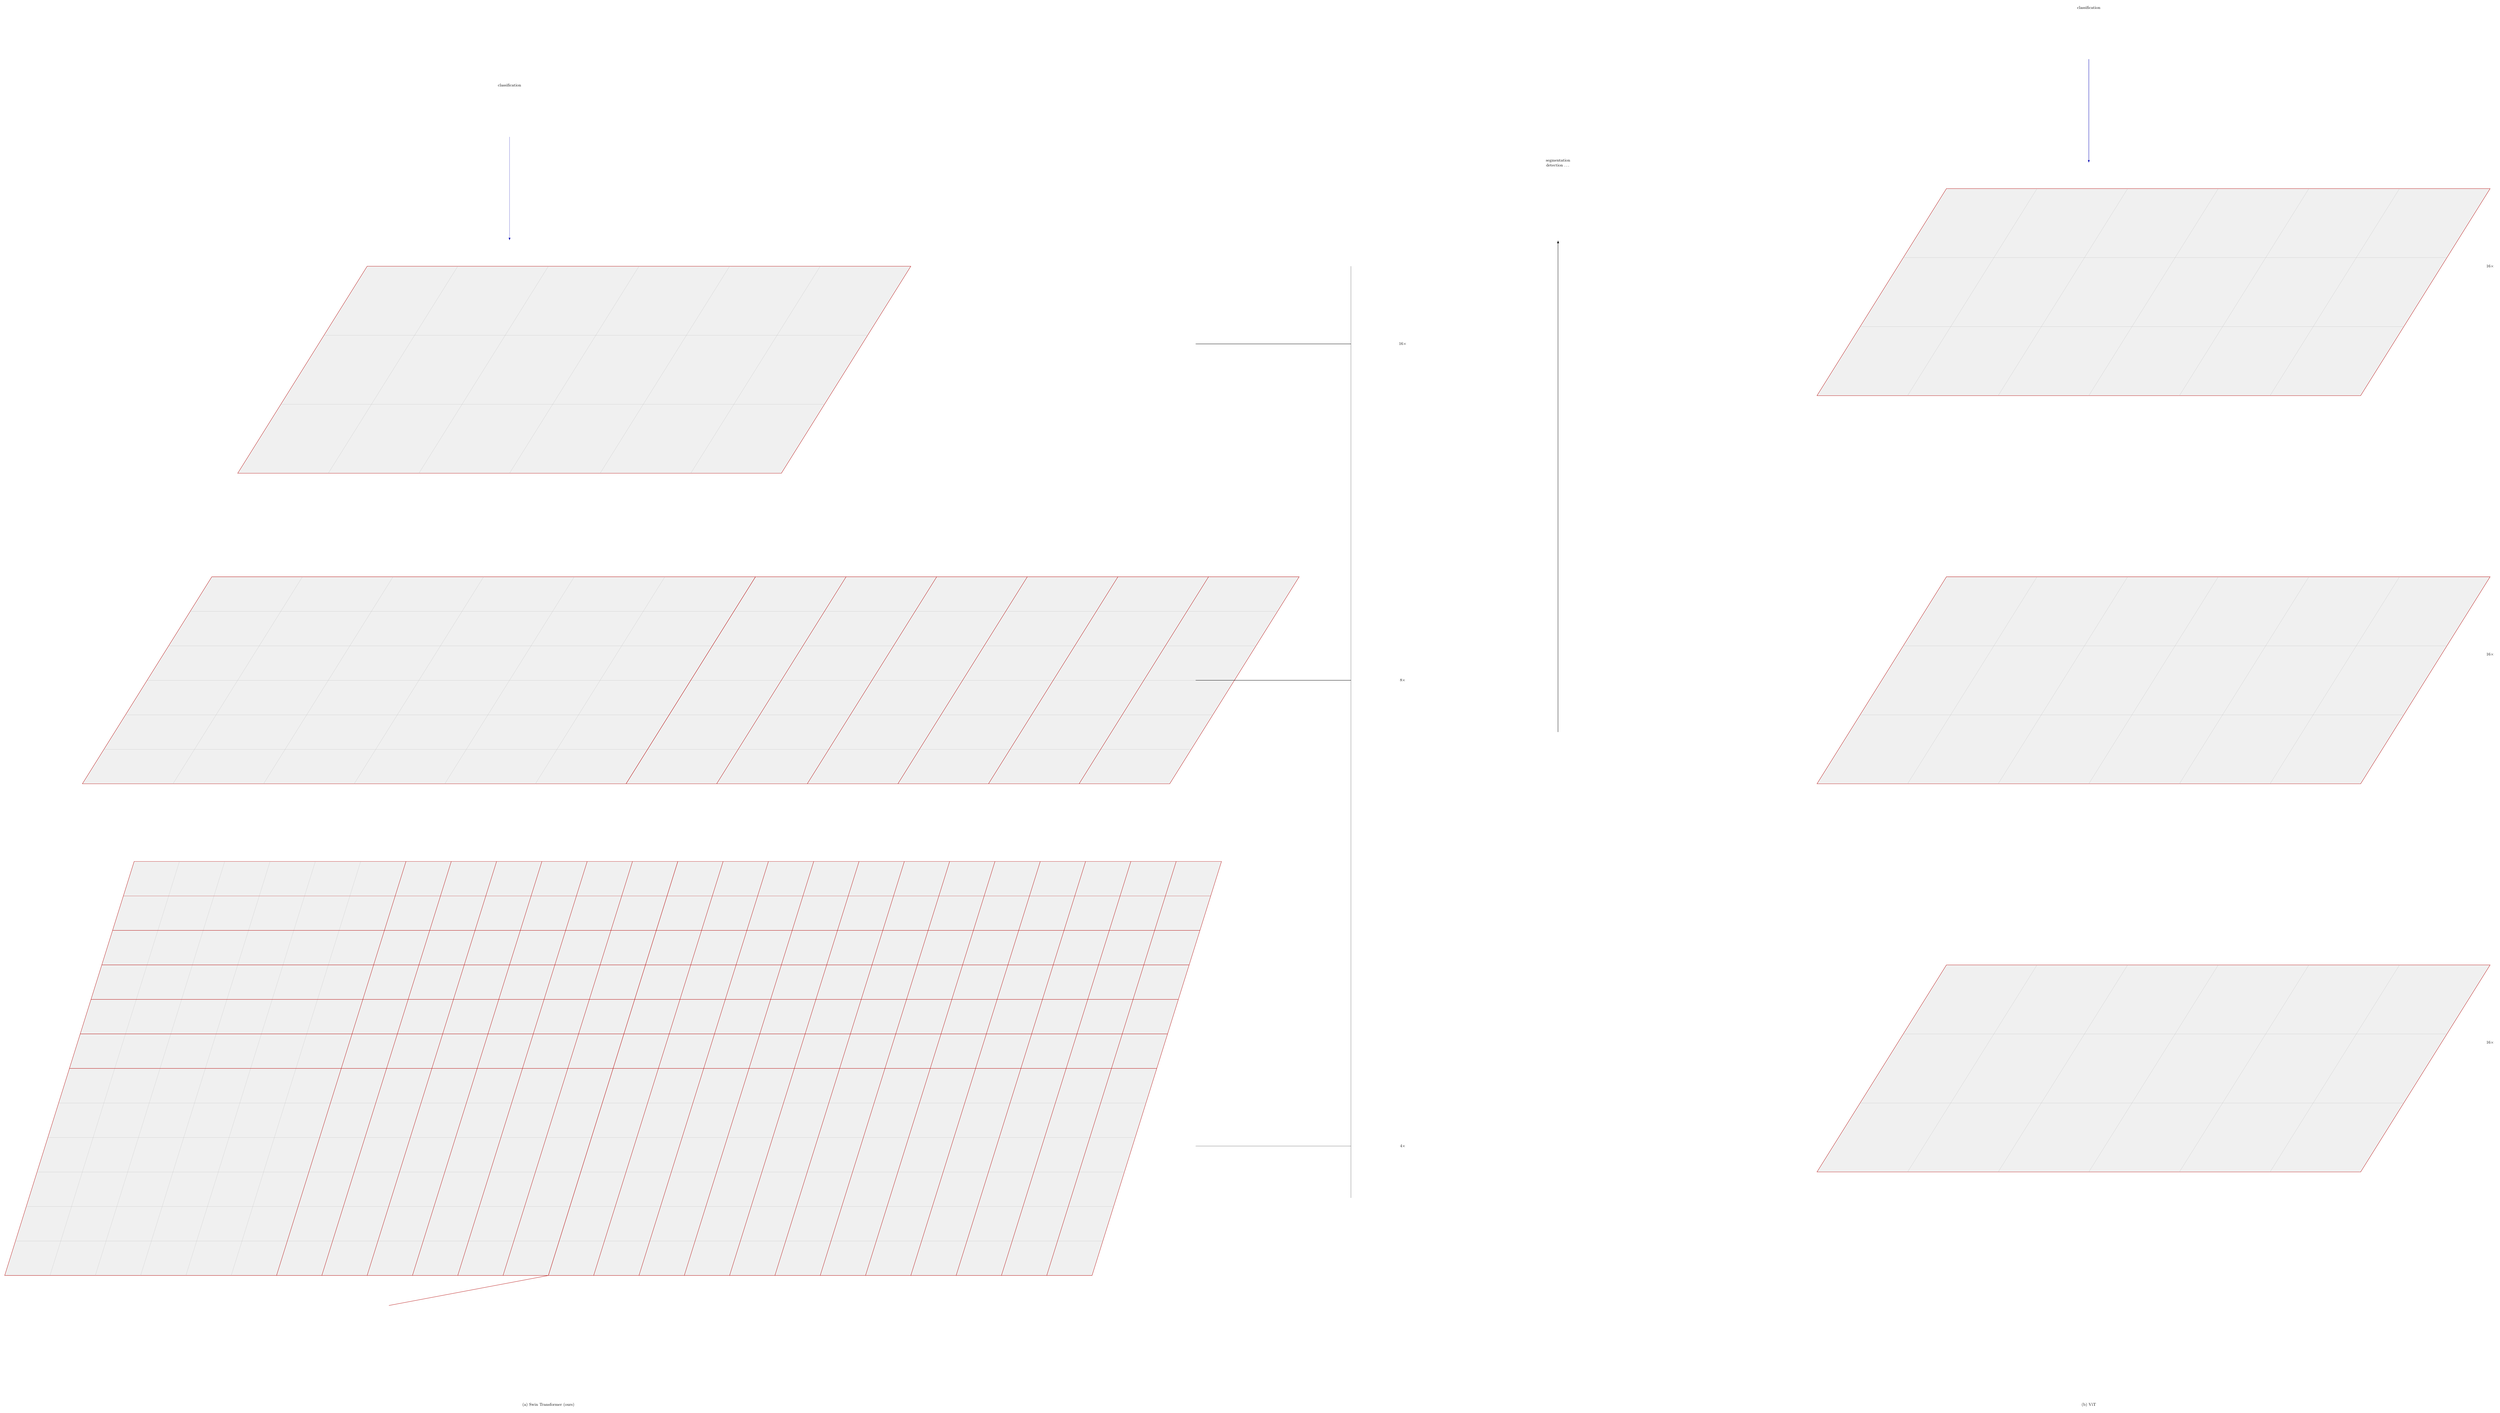
\begin{tikzpicture}[
  font=\small,
  >=Latex,
  outline/.style={draw=red!70!black, line width=0.6pt},
  grid/.style={draw=gray!55, line width=0.25pt},
  win/.style={draw=red!70!black, line width=0.6pt},
  lab/.style={font=\small}
]

% --------- helper: draw a perspective plane with grid + window grid ----------
% args: x,y, W,H, S, nx,ny, wx,wy
\newcommand{\DrawPlane}[9]{%
  \coordinate (A) at (#1,#2);
  \coordinate (B) at ($(A)+(#3,0)$);
  \coordinate (D) at ($(A)+(#5,#4)$);
  \coordinate (C) at ($(B)+(#5,#4)$);

  % fill
  \path[fill=gray!12] (A) -- (B) -- (C) -- (D) -- cycle;
  % outline
  \draw[outline] (A) -- (B) -- (C) -- (D) -- cycle;

  % fine grid (nx, ny)
  \foreach \i in {1,...,#6} {
    \ifnum\i<#6
      \draw[grid] ($(A)!\i/#6!(B)$) -- ($(D)!\i/#6!(C)$);
    \fi
  }
  \foreach \j in {1,...,#7} {
    \ifnum\j<#7
      \draw[grid] ($(A)!\j/#7!(D)$) -- ($(B)!\j/#7!(C)$);
    \fi
  }

  % window boundaries every wx / wy (if >0)
  \ifnum#8>0
    \foreach \i in {#8, ..., #6} {
      \ifnum\i<#6
        \draw[win] ($(A)!\i/#6!(B)$) -- ($(D)!\i/#6!(C)$);
      \fi
    }
  \fi
  \ifnum#9>0
    \foreach \j in {#9, ..., #7} {
      \ifnum\j<#7
        \draw[win] ($(A)!\j/#7!(D)$) -- ($(B)!\j/#7!(C)$);
      \fi
    }
  \fi
}

% =======================
% (a) Swin Transformer
% =======================
% geometry
\def\Skew{10} % skew S

% bottom: 2x2 tiles (big plane)
\DrawPlane{0}{0}{84}{32}{\Skew}{24}{12}{6}{6}
% tile split lines (2x2)
\draw[win] ($(0,0)!0.5!(84,0)$) -- ($(0,\Skew,32)!0.5!(84,\Skew,32)$); % vertical-ish (approx via interpolation)
% easier explicit using plane corners:
\coordinate (Ab) at (0,0);
\coordinate (Bb) at ($(Ab)+(84,0)$);
\coordinate (Db) at ($(Ab)+(\Skew,32)$);
\coordinate (Cb) at ($(Bb)+(\Skew,32)$);
\draw[win] ($(Ab)!0.5!(Bb)$) -- ($(Db)!0.5!(Cb)$);
\draw[win] ($(Ab)!0.5!(Db)$) -- ($(Bb)!0.5!(Cb)$);

% middle: 2 tiles side-by-side
\DrawPlane{6}{38}{84}{16}{\Skew}{12}{6}{6}{6}
\coordinate (Am) at (6,38);
\coordinate (Bm) at ($(Am)+(84,0)$);
\coordinate (Dm) at ($(Am)+(\Skew,16)$);
\coordinate (Cm) at ($(Bm)+(\Skew,16)$);
\draw[win] ($(Am)!0.5!(Bm)$) -- ($(Dm)!0.5!(Cm)$);

% top: 1 tile
\DrawPlane{18}{62}{42}{16}{\Skew}{6}{3}{0}{0}

% classification arrow (left)
\node[lab] (clsL) at ($(18,62)+(21,30)$) {classification};
\draw[->, blue!70!black, line width=0.6pt] ($(18,62)+(21,26)$) -- ($(18,62)+(21,18)$);

% scale bracket + labels (left)
\coordinate (brx) at (104,8);
\draw[line width=0.6pt] (104,6) -- (104,78);
\draw[line width=0.6pt] (104,10) -- (92,10);
\draw[line width=0.6pt] (104,46) -- (92,46);
\draw[line width=0.6pt] (104,72) -- (92,72);
\node[lab] at (108,10) {$4\times$};
\node[lab] at (108,46) {$8\times$};
\node[lab] at (108,72) {$16\times$};

\node[lab] at (42,-10) {(a) Swin Transformer (ours)};

% =======================
% (b) ViT
% =======================
\def\Xvit{140}

% three identical planes (16x each)
\DrawPlane{\Xvit}{8}{42}{16}{\Skew}{6}{3}{0}{0}
\DrawPlane{\Xvit}{38}{42}{16}{\Skew}{6}{3}{0}{0}
\DrawPlane{\Xvit}{68}{42}{16}{\Skew}{6}{3}{0}{0}

% classification arrow (right)
\node[lab] (clsR) at ($(\Xvit,68)+(21,30)$) {classification};
\draw[->, blue!70!black, line width=0.6pt] ($(\Xvit,68)+(21,26)$) -- ($(\Xvit,68)+(21,18)$);

% 16x labels on the right planes
\node[lab] at ($(\Xvit,8)+(52,10)$) {$16\times$};
\node[lab] at ($(\Xvit,38)+(52,10)$) {$16\times$};
\node[lab] at ($(\Xvit,68)+(52,10)$) {$16\times$};

\node[lab] at (\Xvit+21,-10) {(b) ViT};

% =======================
% center arrow: segmentation / detection ...
% =======================
\coordinate (midX) at (120,42);
\draw[->, line width=0.7pt] (midX) -- ($(midX)+(0,38)$);
\node[lab, align=center] at ($(midX)+(0,44)$) {segmentation\\detection \dots};

\end{tikzpicture}
\end{document}
